\beginsong{Der Wagen}[mel={Sergej Kossigin}, txt={Erik Schellhorn (fotler) und Igor Plachonin}, index={Staub, Staub und Steppenland}]

\beginverse
\endverse
\centering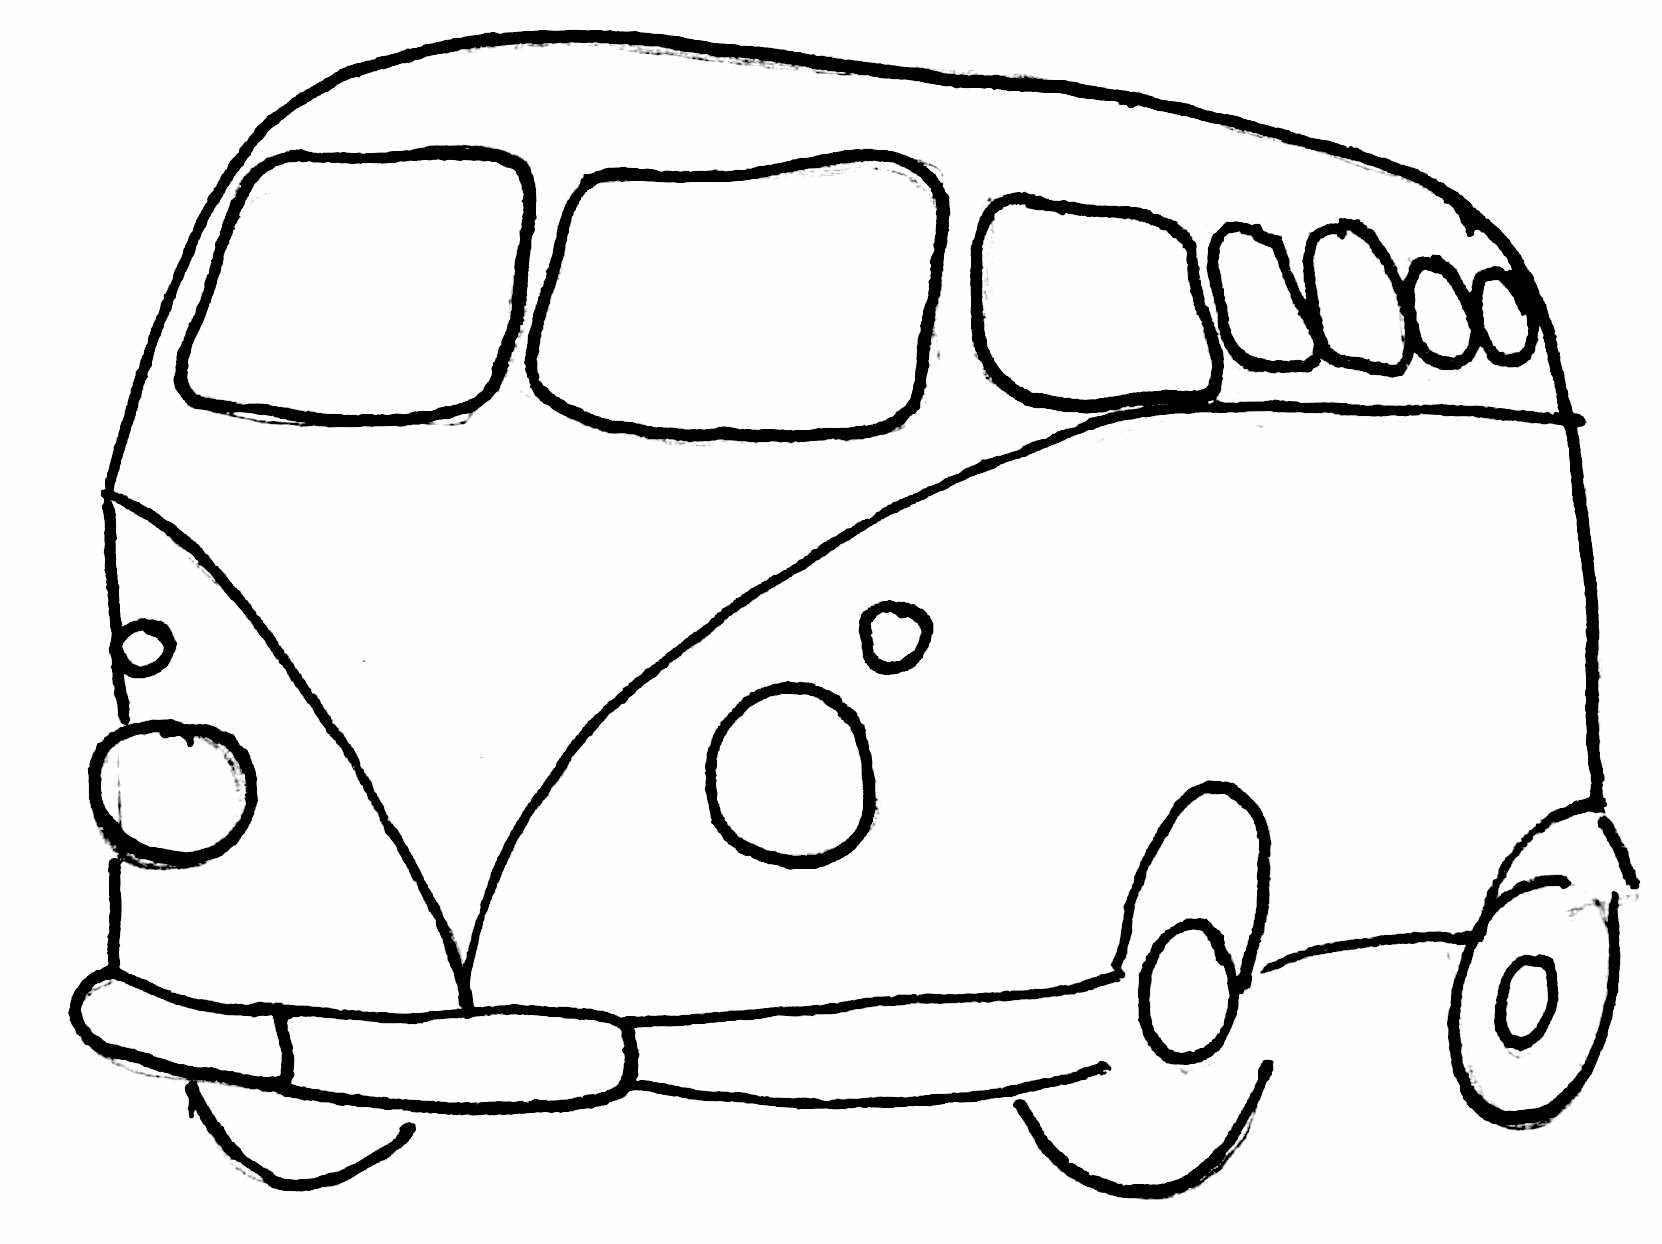
\includegraphics[width=1\textwidth]{Noten/Wagen.pdf}

\beginverse*
\textbf{Zwischenspiel: \\}
\endverse
\centering\includegraphics[width=1\textwidth]{Noten/Wagen-Zwischenspiel.pdf}	


\beginverse\memorize
\[Am]Staub, \[F]Staub \[G]und Steppen\[Am]land, zwei alte \[F]Mulis\[G] am Weges\[Am]rand.
Zieh'n den \[F]Wagen\[G] aus der \[Dm]Stadt, weiter nach \[Am]Osten\[Em] dreht sich das \[Am]Rad.
\endverse

\beginverse
^Glaub', ^glaub',^ mein alter F^reund, vom Glück da ^haben^ wir oft ge^träumt. 
Knarrt das ^Fuhrwe^rk im Sturmge^braus, Die Mulis ^finden^{ nie} mehr nach ^Haus.
\endverse

\beginverse
^Fern, ^fern^ in schwerer ^Stund, hilft nur die ^Kneipe^ am Wiesen^grund.
Die Wahrheit ^ände^rn wir nie^mals, dem Schicksal ^trotzend^{ auf} weiter ^Straß'.
\endverse

\beginverse
^Weit, ^weit^ und grau der ^Weg und unsre ^Stiefel^ steh'n starr vor ^Dreck. 
Die Fahrt vor^bei^, in Träumen ^zieh'n wir im ^Wagen^ nochmals da^hin.
\endverse

\beginverse
^Staub, ^Staub^ und Steppen^land, zwei alte ^Mulis^ am Weges^rand,
zieh'n den ^Wagen^ aus der ^Stadt, weiter nach ^Osten^ dreht sich das ^Rad.
\endverse

\beginverse
^Stjep, ^Stjep^, Stjep kru^gom, Dwa starich ^mula^ vesut fur^gon. 
Iz gorodor ^ot^ suje^ti na Dalni ^zapad^ uchodim ^my.
\endverse

\endsong